%!TEX root=../oi-magistr-si.tex
\setcounter{section}{18}
\section[WA2 - Cloud]{Cloud architektury, virtualizace, různá pojetí cloudových řešení, omezení cloudových aplikací, náklady na provoz, vlastnosti aplikací vhodných pro nasazení v cloud architektuře.}

Cloud-Computing architektury můžeme rozdělit do 3 hlavních vrstev:

\begin{figure}[h!]
\centering
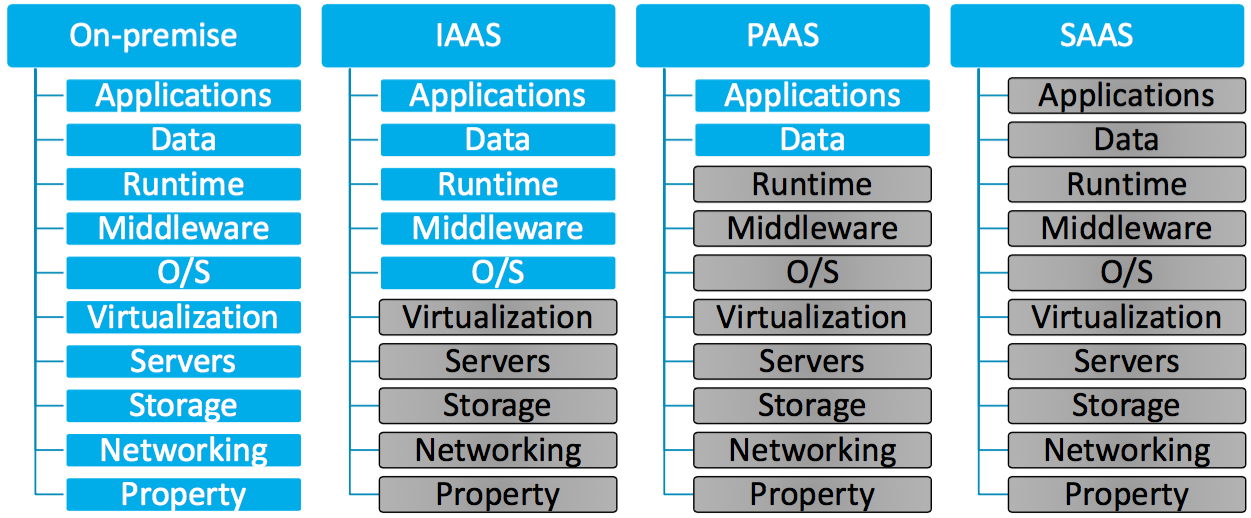
\includegraphics[width=140mm]{19/images/cloud-types}
\end{figure}

\subsection{Infrastructure as a Service (IaaS)}
Je to vlastně outsourcing výpočetního vybavení (servery, HW, síťové komponenty, storage). Poskytovatel služby je odpovědný za housing, běh a správu těchto komponent. Klient obvykle platí v modelu \textit{pay-as-you-go} či smluvním paušálem (předplatným), popřípadě kombinací obojího.
\paragraph{Příklady služeb IaaS:} Amazon EC2, Amazon S3, GTS Managed Server - Virtual Server.

\subsection{Platform as a Service (PaaS)}
Provider poskytuje přístup ke computing platformě či computing stacku (množina softwarových subsystemů, které poskládáte do výsledné služby). Jako v případě IaaS máte k dispozici servery, storage, ale omezené vybranou platformou. Zatímco na IaaS můžete v rámci virtuálního prostředí provozovat téměř jakoukoliv aplikaci, volba platformy (operacniho systemu ci programovaciho jazyka) je plně v kompetenci klienta, u PaaS jste již vázáni kompletní platformou.

\paragraph{Nebezpečí Vendor Lock-In} jste omezeni platformou poskytovate (.NET na MS Azzure), proprietární službou či množinou podporovaných programovacích jazyků. Flexibilita služby nemusí stačit rapidně se vyvyjejícím projektům (paměťové limity, model automatického deploymentu).

\paragraph{Příklady služeb PaaS} Google App Engine (platforma: Java, Python, Go), MS Azure (platforma: .NET, Ruby, Java, PHP).

\subsection{Software as a Service (SaaS)}
Model pronájmu hotových aplikací, které jsou k dispozici klientovi skrze interface (nejčastěji kombinace REST+JSON) či uživatelské rozhraní (Facebook, YouTube, BaseCampHQ, Google Apps.. ).
\paragraph{Příklady aplikací SaaS} Google Apps, E-mail, Kalendář, Microsoft Live

\subsection{Omezení cloudu}
\begin{itemize}[itemsep=0px]
\item v \textbf{bezpečnosti} spoléháme na dodavatele cloudu
\item \textbf{zneužití} - můžu si pronajmout cloud a udělat DDOS útok
\item \textbf{legislativa} - např. některé evropské země nedovolují ukládání osobních informací mimo EU
\item \textbf{copyright} - nesmíte přenášet copyrightované materiály mimo zemi licence
\end{itemize}

\subsection{Náklady na provoz}
\paragraph{Pay-As-You-Go} - Platíte pouze za spotřebované zdroje (použité storage, vypočetní čas, traffic). Obvykle 0 upfront investment. Konsolidovaná fakturace (denní, týdenní, .. vyúčtování za použité služby na jednom účtu). Cena zahrnuje náklady na:
\begin{itemize}[itemsep=0px]
\item hardware
\item údržba
\item utitilies
\item případné SW licence
\end{itemize}
Vendor uplatnuje obvykle economies-of-scale (jenotkove mensi naklady na MB storage, traffic, hodinu procesoroveho casu... )

\paragraph{Paušál} Můžete si \textbf{předplatit} určitý počet hodin procesorového času. Paušál za měsíční provoz virtual serveru atd..

\subsection{Virtualizace}
Virtualizace je technika (postup) přístupu ke zdrojům jiným způsobem, než jsou fyzicky zapojeny. Dá se virtualizovat \textbf{celý stroj} (VirtualBox, Vmware, Microsoft Virtual PC, Android emulátor), \textbf{jednotlivé komponenty} (např. RAID se navenek tváří jako jeden disk, virtuální paměť může naalokovat více paměti než je fyzicky dostupné, ...), jiný \textbf{systém} (Wine v Linuxu, NTFS driver v Linuxu), aplikace (JVM, .NET VM). Virtualizace je ekonomicky výhodná, centrálně spravovatelná, bezpečná (když uživatel něco provede naloadujeme čistý image), odděluje logiku od konkrétního hardware.

\begin{itemize}[itemsep=0px]
\item emulace nebo simulace - VM simuluje celý hardware, dovoluje běh neupraveného OS na zcela odlišném hardware (Microsoft Virtual PC, AVD emulator pre Android)
\item nativní (plná) virtualizace - VM simuluje dostatečné množství komponent, aby umožnil běh neupraveného OS (VMware, VirtualBox, Parallels)
\item částečná virtualizace - VM simuluje instance mnoha prostředí, na kterém běží hostitel - Linux, MS Windows
\item paravirtualizace - VM nesimuluje HW ale nabízí API (hypercall), přes které se komunikuje (Xen)
\item virtualizace na úrovni operačního systému
\item aplikační virtualizace
\end{itemize}

\subsection{Vhodné aplikace pro cloud}
Nové weby, které nejsou svázány konkrétní databází/technologií. Malé weby, které v cloudu můžou běžet i zadarmo. Globální weby, které potřebují hodně škálovat a mít nízkou latenci všude po světě. Aplikace které nejsou primárně sekvenční a využijí paralelizaci. Weby které potřebují pracovat s obrovskými daty. Eshopy, které se většinu roku flákají a pak před Vánocemi to přijde.